%%%%%%%%%%%%%%%%%%%%%%%%%%%%%%%%%%%%%%%%%%%%%%%%%%%%%%%%%%%%%%%%%%%%%%
% Skupina21/main.tex -- Tara Majkič, Jaka Pelko in Miha Vintar
%%%%%%%%%%%%%%%%%%%%%%%%%%%%%%%%%%%%%%%%%%%%%%%%%%%%%%%%%%%%%%%%%%%%%%

\graphicspath{{Skupina21/img/}}

\title{Enoplastni fizično reverzibilni demultiplekser s sinhronimi izhodi v QCA}
\author{Tara Majkič, Jaka Pelko in Miha Vintar}
\maketitle

\abstract{
V seminarski nalogi smo raziskovali, ali je mogoče zasnovati enoplastni logično in fizično reverzibilni demultiplekser 1:2 brez križanja vodil in s sinhronimi izhodi. V simulatorju QCADesigner-E smo rekonstruirali dve obstoječi vezji in zasnovali dve lastni različici. Njihovo delovanje in energijsko disipacijo smo preverili pri dveh hitrostih ure ter primerjali število celic, površino, zakasnitev in ceno. Končna sinhrona različica vsebuje 63 celic in ima zakasnitev 1,25 urinega cikla. Pri desetkrat počasnejši uri se je njena energijska disipacija zmanjšala za 9,7-krat na 0,00790 meV, kar je pod Landauerjevo mejo. Rezultati kažejo, da je mogoče fizično reverzibilnost združiti z enoplastno izvedbo in sinhronimi izhodi, vendar pri večji površini in energijski disipaciji.
}

\section{Uvod}
\label{g21:sec:uvod}

Demultiplekserji so pomembni gradniki digitalnih vezij, ki se uporabljajo za usmerjanje podatkovnih signalov. Njihova realizacija je mogoča tudi s tehnologijo kvantnih celičnih avtomatov, pri katerih je eden izmed pomembnih izzivov zmanjševanje energijske disipacije. V seminarski nalogi obravnavamo zasnovo enoplastnega fizično reverzibilnega demultiplekserja s sinhronimi izhodi ter primerjamo njegove lastnosti z obstoječimi izvedbami.

\subsection{Demultiplekser}
\label{g21:sec:demux}

Demultiplekser (angl. \emph{demultiplexer}) je kombinacijsko logično vezje, ki omogoča usmerjanje podatkovnega signala z enega vhoda na enega izmed več izhodov. Kateri izhod prejme vhodni signal, določajo izbirni vhodi. Število izhodov je odvisno od števila izbirnih vhodov in je enako $2^n$, kjer je $n$ število izbirnih vhodov~\cite{g21:dsouza2026}.

Najpreprostejša različica je demultiplekser 1:2, ki ima en podatkovni vhod, en izbirni vhod in dva izhoda. Njegovo delovanje je prikazano v tabeli~\ref{g21:tab:demux}.

\begin{table}[htbp]
    \centering
    \caption{Pravilnostna tabela demultiplekserja 1:2.}
    \label{g21:tab:demux}
    \begin{tabular*}{0.25\linewidth}{@{\extracolsep{\fill}}cccc}
        \toprule
        $S$ & $DATA$ & $Y_0$ & $Y_1$ \\
        \midrule
        0 & 0 & 0 & 0 \\
        0 & 1 & 0 & 1 \\
        1 & 0 & 0 & 0 \\
        1 & 1 & 1 & 0 \\
        \bottomrule
    \end{tabular*}
\end{table}

Pri izbirnem vhodu $S=0$ se podatkovni signal prenese na izhod $Y_1$, pri $S=1$ pa na izhod $Y_0$. Izhod, ki ni izbran, ima v obeh primerih vrednost 0.


\subsection{Kvantni celični avtomati}
\label{g21:sec:qca}

Kvantni celični avtomati (angl. \emph{Quantum-dot Cellular Automata}, QCA) predstavljajo eno izmed možnih alternativ tehnologiji CMOS, saj za predstavitev in prenos informacij namesto tranzistorskega preklapljanja uporabljajo medsebojne elektrostatične interakcije med kvantnimi celicami~\cite{g21:janez2012}.

Osnovni gradnik QCA je celica z dvema elektronoma in štirimi kvantnimi pikami, razporejenimi v oglišča kvadrata. Zaradi medsebojnega Coulombovega odboja se elektrona razporedita na dve diagonalno nasprotni kvantni piki. Ti dve možni razporeditvi predstavljata logični vrednosti 0 in 1~\cite{g21:janez2012}.

Procesiranje v QCA temelji na tuneliranju elektronov med kvantnimi pikami znotraj posamezne celice. Na njihovo razporeditev vplivajo elektrostatične interakcije s sosednjimi celicami, zaradi katerih se elektroni razporedijo tako, da je skupna elektrostatična energija sistema čim manjša. Z ustrezno razporeditvijo večjega števila celic tako omogočimo prenos informacij in izvajanje logičnih operacij~\cite{g21:janez2012}.

Za nadzorovano preklapljanje stanj kvantnih celic uporabljamo urin signal, ki uravnava višino potencialnih pregrad med kvantnimi pikami in s tem omogoča oziroma omejuje tuneliranje elektronov. Takšno krmiljenje omogoča postopno prehajanje med stanji in zmanjšuje možnost, da bi sistem zašel v metastabilno stanje. Urin signal sestavljajo štiri faze: preklop, zadrževanje, sproščanje in sproščenost~\cite{g21:janez2012}.

\subsection{Logična in fizična reverzibilnost}
\label{g21:sec:reverzibilnost}

Konvencionalne metode procesiranja pogosto vključujejo ireverzibilne operacije, pri katerih se informacije o vhodnih podatkih med procesiranjem nepovratno izgubijo. Pri izbrisu enega bita informacije se v okolico sprosti toplota, katere najmanjša vrednost je določena z Landauerjevim načelom~\cite{landauer1961,g21:alharbi2023alu}.

Pri načrtovanju QCA-vezij si prizadevamo za čim manjšo energijsko disipacijo, saj lahko sproščanje toplote negativno vpliva na njihovo delovanje in zanesljivost. Eden izmed pristopov k zmanjšanju energijske disipacije je uporaba reverzibilnih vezij~\cite{g21:alharbi2023alu}. 

Vezje je logično reverzibilno, če lahko iz njegovih izhodnih vrednosti enolično določimo vhodne. Vendar logična reverzibilnost sama po sebi še ne zagotavlja fizične reverzibilnosti, ker lahko med delovanjem vezja prihaja do nepovratnega brisanja informacij. Fizična reverzibilnost zahteva, da se informacije ne izgubljajo niti med samim izvajanjem logičnih operacij. To lahko dosežemo z ustrezno zasnovo vezja, ki informacije ohranja tudi med preklapljanjem stanj celic. Pri fizično reverzibilnih vezjih lahko z dovolj počasnim preklapljanjem zmanjšujemo energijsko disipacijo in se v idealnih pogojih približujemo ničelni disipaciji~\cite{g21:alharbi2023alu}.

\subsection{Obstoječe rešitve in raziskovalno vprašanje}
\label{g21:sec:resitve}

Na področju QCA je bilo razvitih več izvedb demultiplekserjev, ki se razlikujejo po kompleksnosti, energijski disipaciji ter logični in fizični reverzibilnosti.

Ena izmed njih je demultiplekser 1:2 Aswathyja in sod.~\cite{g21:aswathy2024}, ki ga odlikujeta majhno število celic in razmeroma nizka energijska disipacija. Vendar vezje ni niti logično niti fizično reverzibilno, kar povzroča neizogibno energijsko disipacijo v skladu z Landauerjevim načelom.

Drugačen pristop so predstavili Alharbi in sod.~\cite{g21:alharbi2022}, ki so zasnovali logično in fizično reverzibilni demultiplekser 1:2. Vendar njihova izvedba zahteva večplastno križanje vodil, poleg tega pa izhodi niso časovno sinhronizirani.

\begin{svgraybox}
\textbf{Raziskovalno vprašanje.}
Ali je mogoče zasnovati enoplastni logično in fizično reverzibilni demultiplekser 1:2 brez križanja vodil in s sinhronimi izhodi?

\medskip
\textbf{Pričakovani rezultat.}
Pričakujemo, da je z ustrezno razporeditvijo QCA-celic in urinih con mogoče odpraviti večplastno križanje vodil ter doseči sinhronost izhodov ob ohranitvi logične in fizične reverzibilnosti.
\end{svgraybox}

V nadaljevanju najprej predstavimo uporabljena orodja, zasnovo poskusov in metodologijo meritev. Nato primerjamo rezultate simulacij glede na zgradbo vezij, sinhronost izhodov in energijsko disipacijo. Sledi razprava, v kateri ovrednotimo rezultate in predstavimo omejitve raziskave, v zaključku pa povzamemo glavne ugotovitve in možnosti nadaljnjih izboljšav.

\section{Metode}
\label{g21:sec:metode}

V tem poglavju opišemo, kako smo načrtovali, simulirali in ovrednotili vezja demultiplekserja 1:2. Najprej v razdelku~\ref{g21:sec:orodja} navedemo uporabljena orodja in vse nastavitve simulacije, ki vplivajo na rezultate. Nato v razdelku~\ref{g21:sec:poskusi} opišemo primerjana vezja in poskuse, s katerimi smo preverili njihovo pravilnost, ocenili disipacijo energije in poiskali znake fizične reverzibilnosti. Na koncu v razdelku~\ref{g21:sec:metrike} definiramo metrike, s katerimi vezja primerjamo med seboj.

\subsection{Orodja in nastavitve}
\label{g21:sec:orodja}

Vsa vezja smo načrtovali in simulirali v simulatorju QCADesigner-E~\cite{walus2004,silltorres2018}, različica 2.2. V simulator smo dodali lastne popravke, ki zmanjšajo število sesutij simulatorja. Prav tako smo dodali ukaz \emph{Reset Polarization}, ki odstrani polarizacijo celic, kar omogoča izvoz preglednejših slik. Popravki ne posegajo v izračun simulacije, zato ne vplivajo na rezultate.

Simulator smo prevedli in zagnali v vsebniku Docker z orodjem Docker Compose. Tako smo zagotovili ponovljivo razvojno okolje. Slike vezij in grafe valovnih oblik smo iz simulatorja izvozili kot PostScript. Pred izvozom smo polarizacijo celic ponastavili s prej omenjeno dodano funkcionalnostjo. Datoteke PostScript smo nato pretvorili v format PDF. Diagrame energije smo narisali v Pythonu s knjižnico matplotlib.

Vse meritve smo izvedli s pogonom \emph{Coherence Vector (w/ Energy)} v načinu \emph{Exhaustive Verification}, ki zaporedoma preizkusi vse kombinacije vhodov. Alharbi in sod.~\cite{g21:alharbi2022} so namesto tega uporabili tabelo vektorjev s kombinacijami vhodov 00, 01, 10 in 11. Pogon \emph{Bistable Approximation} smo uporabili le za hitro preverjanje logike med načrtovanjem, saj energije ne računa. Fizikalne nastavitve so bile pri vseh simulacijah enake (tabela~\ref{g21:tab:parametri}) in se, razen nastavitve \emph{Zeroing of Inputs}, ujemajo z nastavitvami Alharbija in sod.

\begin{table}[htbp]
\centering
\caption{Nastavitve pogona \emph{Coherence Vector (w/ Energy)}, enake pri vseh simulacijah.}
\label{g21:tab:parametri}
\begin{tabular*}{0.85\linewidth}{@{\extracolsep{\fill}}lr}
\toprule
Parameter & Vrednost \\
\midrule
temperatura (\emph{Temperature}) & \SI{1}{\kelvin} \\
velikost kvantne pike (\emph{Dot diameter}) & \SI{5}{\nano\metre} \\
širina celice (\emph{Cell width}) & \SI{18}{\nano\metre} \\
višina celice (\emph{Cell height}) & \SI{18}{\nano\metre} \\
razdalja med središči celic (\emph{Grid spacing}) & \SI{20}{\nano\metre} \\
relaksacijski čas (\emph{Relaxation Time}) & \SI{1e-15}{\second} \\
časovni korak (\emph{Time Step}) & \SI{1e-16}{\second} \\
visoka vrednost ure (\emph{Clock High}) & \SI{9.8e-22}{\joule} \\
nizka vrednost ure (\emph{Clock Low}) & \SI{3.8e-23}{\joule} \\
zamik ure (\emph{Clock Shift}) & \num{0} \\
oblika urinega signala (\emph{GAUSS ali RAMP}) & GAUSS \\
radij vpliva (\emph{Radius of Effect}) & \SI{80}{\nano\metre} \\
relativna dielektričnost (\emph{Relative Permittivity}) & \num{12.9} \\
razmik med plastmi (\emph{Layer Separation}) & \SI{11.5}{\nano\metre} \\
numerična metoda (\emph{Euler ali Runge Kutta}) & Euler \\
naključni vrstni red simuliranja (\emph{Randomize Simulation Order}) & vklopljeno \\
ničenje vhodov (\emph{Zeroing of Inputs}) & vklopljeno \\
\bottomrule
\end{tabular*}
\end{table}

Nastavitev \emph{Zeroing of Inputs} vhodno celico pred vsako novo vrednostjo za pol cikla postavi na 0 in tako posnema zadnjo celico predhodnega vezja z uro. Alharbi in sod.~\cite{g21:alharbi2022} so jo imeli izklopljeno. Preverili smo, da njen vpliv na disipacijo energije znaša manj kot \SI{1}{\percent} (\SI{0.0704}{\milli\electronvolt} z njo in \SI{0.0710}{\milli\electronvolt} brez nje, Alharbijevo vezje s testnim okoljem pri \SI{10}{\pico\second}).

Vsako vezje smo simulirali pri dveh hitrostih ure, ki ju poimenujemo po času prehoda ure (\emph{Clock Slope}): pri \SI{100}{\pico\second}, kot Alharbi in sod.~\cite{g21:alharbi2022}, in pri desetkrat hitrejši uri \SI{10}{\pico\second}. Perioda ure (\emph{Clock Period}) je enaka periodi vhodov (\emph{Input Period}) in je desetkratnik časa prehoda ure, simulacija pa traja 8 period.

Energijo smo merili v testnem okolju po Sill Torresu in sod.~\cite{silltorres2018}: pred vsak vhod in za vsak izhod vezja smo dodali po 4 medpomnilniške celice z vklopljeno nastavitvijo \emph{Ignore Energy Dissipation}, zato se v disipacijo energije ne štejejo.

\subsection{Zasnova poskusov}
\label{g21:sec:poskusi}

Cilj naloge je bil izboljšati obstoječa demultiplekserja 1:2. Vezje Aswathyja in sod.~\cite{g21:aswathy2024} je enoplastno, vendar ni reverzibilno, zato njegove disipacije energije ni mogoče znižati pod Landauerjevo mejo. Vezje Alharbija in sod.~\cite{g21:alharbi2022} je fizično reverzibilno, a za križanje žic potrebuje več plasti. To je pomembna ovira, saj se tehnologije FCN (\emph{field-coupled nanocomputing}), kamor spada QCA, izdelujejo v eni plasti, križanja žic pa poleg tega ogrožajo stabilnost signala~\cite{g21:hien2025}. Zato smo zasnovali dve lastni različici, ki sta hkrati enoplastni in fizično reverzibilni: nesinhrono in sinhrono, pri kateri so vsi izhodi na voljo ob istem času. Vsa štiri vezja smo primerjali pod enakimi pogoji, da ugotovimo, ali lastni različici kažeta znake fizične reverzibilnosti in kakšna je cena izboljšave v disipaciji energije, površini in zakasnitvi.

Najprej smo ponovili obe referenčni vezji. Rezultati iz člankov med seboj niso neposredno primerljivi, saj so dobljeni z različnimi orodji in nastavitvami, zato smo vezji narisali po slikah iz člankov in ju simulirali sami. Pravilnost rekonstrukcije smo preverili z ujemanjem z objavljenimi rezultati: pri Aswathyjevem vezju z disipacijo energije, pri Alharbijevem pa z zakasnitvami izhodov, številom ploščic in disipacijo energije.

Na fizično reverzibilnost smo sklepali iz disipacije energije pri dveh hitrostih ure, \SI{10}{\pico\second} in \SI{100}{\pico\second}, saj se disipacija energije fizično reverzibilnega vezja ob različnih hitrostih ure občutno spremeni, poraba ireverzibilnega pa ne. Zaradi dolgega časa izvajanja simulacij smo meritve izvedli le pri teh dveh hitrostih. Glavne meritve smo izvedli v testnem okolju. V njem izhodi niso zadnje celice, zato se njihova vrednost ne izbriše in lahko izmerimo disipacijo energije samega vezja. Aswathyjevemu vezju testnega okolja ni mogoče dodati, ker vhod $S$ obdajajo druge celice. Zato smo vsa vezja izmerili tudi brez testnega okolja, kar omogoča primerjavo pod enakimi pogoji in pokaže, koliko energije stane brisanje informacije na izhodih.

Pravilnost delovanja in sinhronost izhodov sinhrone različice smo preverili še z grafom valovnih oblik.

\subsection{Metrike}
\label{g21:sec:metrike}

Vsa vezja smo narisali v QCADesigner-E, ki jih shrani v datoteke \texttt{.qca}: referenčni vezji po slikah iz člankov, lastni različici pa smo zasnovali sami. Metrike razen energije smo izračunali iz teh datotek brez testnega okolja, pri Aswathyjevem vezju pa smo jih povzeli iz članka~\cite{g21:aswathy2024}. Število plasti pokaže, ali je vezje enoplastno, razmerje disipacij energije pri dveh hitrostih ure nakazuje, ali je fizično reverzibilno, ostale metrike pa kažejo, kakšna je cena izboljšave.

Zgradbo vezja opišemo s številom plasti, številom celic in površino. Število celic $N$ vključuje vhodni in fiksni celici, pri Alharbijevem vezju pa tudi celice križanja. Površina $A$ je najmanjši pravokotnik okoli vseh celic, kot ga izpiše QCADesigner. V realnem vezju uro ustvarjajo elektrode pod celicami, ki jih ni mogoče narediti za vsako celico posebej, zato se ravnina razdeli na ploščice, v katerih so vse celice v isti urini coni. Pri postavitvi po ploščicah velikosti $5\times5$ celic navedemo še število ploščic, ki merijo po \SI{0.01}{\micro\metre\squared}, in preverimo, ali imajo vse celice v posamezni ploščici isto cono ure.

Zakasnitev izhoda $D$ v urinih ciklih določa enačba~\eqref{g21:eq:zakasnitev}, kjer je $n_\mathrm{con}$ število urinih con na najdaljši poti od vhoda do izhoda, vključno s cono vhoda:
\begin{equation}
D = \frac{n_\mathrm{con}}{4}.
\label{g21:eq:zakasnitev}
\end{equation}
Kritična zakasnitev je največja med izhodi. Izhodi so sinhroni, če imajo vsi enako zakasnitev.

Disipacijo energije merimo s povprečno disipacijo na urin cikel $\bar{E}$ (v simulatorju Avg\_Ebath), ki jo določa enačba~\eqref{g21:eq:avg}, kjer je $E_k$ energija, oddana v okolico v ciklu $k$, in $M = 7$ število vrednosti, ki jih simulator izpiše pri 8 ciklih:
\begin{equation}
\bar{E} = \frac{1}{M}\sum_{k=1}^{M} E_k.
\label{g21:eq:avg}
\end{equation}
Vhodnih, fiksnih in celic z \emph{Ignore} simulator ne šteje, ostale pa imenujemo računane celice in njihovo število označimo z $N_\mathrm{r}$.

Disipacijo energije primerjamo z Landauerjevo mejo, tj.\ najmanjšo energijo, ki se sprosti ob izbrisu enega bita informacije~\cite{landauer1961}. Določa jo enačba~\eqref{g21:eq:landauer}, kjer je $k_\mathrm{B}$ Boltzmannova konstanta, $T$ temperatura, $\ln(2)$ pa izhaja iz tega, da izbris bita zmanjša število možnih stanj z dveh na eno:
\begin{equation}
E_\mathrm{L} = k_\mathrm{B} T \ln(2) = \SI{0.0597}{\milli\electronvolt} \quad \text{pri } T = \SI{1}{\kelvin}.
\label{g21:eq:landauer}
\end{equation}
Fizično reverzibilnost ocenimo z razmerjem disipacij energije pri obeh hitrostih ure, ki ga določa enačba~\eqref{g21:eq:razmerje}:
\begin{equation}
R = \frac{\bar{E}(\SI{10}{\pico\second})}{\bar{E}(\SI{100}{\pico\second})}.
\label{g21:eq:razmerje}
\end{equation}
Razmerje blizu 10 je skladno s fizično reverzibilnim vezjem, razmerje blizu 1 pa z ireverzibilnim.

Za razlago razlik v disipaciji energije med reverzibilnimi vezji odvisnost $\bar{E}$ od $N_\mathrm{r}$ opišemo s premico skozi izhodišče $\bar{E} = k N_\mathrm{r}$, kjer je naklon $k$ povprečna disipacija na računano celico. Določimo ga po metodi najmanjših kvadratov z enačbo~\eqref{g21:eq:naklon}, kjer indeks $i$ teče po reverzibilnih vezjih:
\begin{equation}
k = \frac{\sum_i N_{\mathrm{r},i}\,\bar{E}_i}{\sum_i N_{\mathrm{r},i}^2}.
\label{g21:eq:naklon}
\end{equation}

Ceno vezja računamo po Aswathyju in sod.~\cite{g21:aswathy2024} z enačbo~\eqref{g21:eq:cena}, kjer je $N$ število celic, $A$ površina v \si{\micro\metre\squared}, $D$ pa kritična zakasnitev v ciklih:
\begin{equation}
C = N \cdot A \cdot D.
\label{g21:eq:cena}
\end{equation}
Ker je število celic že posredno zajeto v površini, navajamo še $A \cdot D^2$.

\section{Rezultati}
\label{g21:sec:rezultati}

V tem poglavju najprej predstavimo zgradbo vseh štirih vezij, nato pokažemo, da ima sinhrona različica vse izhode na voljo ob istem času, na koncu pa primerjamo disipacijo energije.

\subsection{Zgradba vezij}
\label{g21:sec:zgradba}

Slika~\ref{g21:fig:aswathy} prikazuje ireverzibilno vezje Aswathyja in sod.~\cite{g21:aswathy2024}. Vezje nima odmevov vhodov, zato se vrednosti vhodov ob sprostitvi njihove urine cone izbrišejo. Simulacija s privzetimi časovnimi nastavitvami simulatorja da natanko disipacijo energije iz članka (\SI{8.31}{\milli\electronvolt} skupno in \SI{0.755}{\milli\electronvolt} povprečno), kar potrjuje pravilnost rekonstrukcije. Ti vrednosti služita le preverbi, v nadaljnjih primerjavah pa uporabljamo meritve pri urah \SI{10}{\pico\second} in \SI{100}{\pico\second}.

\begin{figure}[htbp]
\centering

\includegraphics[width=0.45\linewidth]{aswathy}
\caption{Ireverzibilni demultiplekser Aswathyja in sod.~\cite{g21:aswathy2024}.}
\label{g21:fig:aswathy}
\end{figure}

Slika~\ref{g21:fig:alharbi} prikazuje rekonstrukcijo fizično reverzibilnega vezja Alharbija in sod.~\cite{g21:alharbi2022}. Fiksna celica levih majoritetnih vrat je na njihovi levi strani, zato mora izhod $Y_0$ najprej v desno in nato navzgor čez žico vhoda $S$. To križanje je izvedeno v dveh dodatnih plasteh s sedmimi celicami. Zakasnitve izhodov in število ploščic se ujemajo s člankom. Disipacija energije pri \SI{100}{\pico\second} s testnim okoljem znaša \SI{0.00759}{\milli\electronvolt}, kar je približno \SI{26}{\percent} več od vrednosti \SI{0.006}{\milli\electronvolt} v članku. Ti dve števili se torej ujemata le po velikostnem redu. Od nastavitev iz članka se razlikujeta le nastavitev \emph{Zeroing of Inputs}, katere vpliv smo izključili, in način simulacije (razdelek~\ref{g21:sec:orodja}). Domnevamo, da razlika izvira iz načina simulacije ali iz nastavitev, ki jih članek ne navaja.

\begin{figure}[htbp]
\centering

\includegraphics[width=\linewidth]{alharbi}
\caption{Rekonstrukcija fizično reverzibilnega demultiplekserja Alharbija in sod.~\cite{g21:alharbi2022}. Celice križanja v drugih plasteh so izrisane kot polni kvadrati.}
\label{g21:fig:alharbi}
\end{figure}

Pri lastni nesinhroni različici (slika~\ref{g21:fig:nesinhroni}) je fiksna celica levih majoritetnih vrat na njihovi desni strani. Izhod $Y_0$ zato vodi naravnost v levo, v novo ploščico, zato je vezje v eni plasti brez križanja. Zasede eno ploščico več kot Alharbijevo vezje. Ker je pot do $Y_0$ krajša, ta izhod pride tri urine cone prej kot ostali.

\begin{figure}[htbp]
\centering

\includegraphics[width=\linewidth]{enoplastni_nesinhroni}
\caption{Lastna enoplastna nesinhrona različica.}
\label{g21:fig:nesinhroni}
\end{figure}

Pri lastni sinhroni različici (slika~\ref{g21:fig:sinhroni}), ki je prav tako v eni plasti, je pot do $Y_0$ podaljšana za tri urine cone. Iz vrat vodi v ploščico na levi (cona 1), nato navzgor (cona 2), v levo (cona 3) in navzdol (cona 0) do izhoda. Vsaka cona je ena ploščica s petimi celicami, pot pa je zložena v kvadrat $2\times2$ ploščic. Navpična dela poti sta pet celic narazen, da med njima ne pride do presluha. Pri vseh treh reverzibilnih vezjih imajo vse celice v posamezni ploščici isto urino cono, zato so vsa izvedljiva s ploščicami $5\times5$.

\begin{figure}[htbp]
\centering

\includegraphics[width=\linewidth]{enoplastni_sinhroni}
\caption{Lastna enoplastna sinhrona različica. Pot do izhoda $Y_0$ je podaljšana za tri ploščice $5\times5$.}
\label{g21:fig:sinhroni}
\end{figure}

Tabela~\ref{g21:tab:zgradba} povzema zgradbo vseh štirih vezij. Aswathyjevo vezje je daleč najmanjše, najhitrejše in najcenejše, vendar je ireverzibilno. Med reverzibilnimi vezji ima nesinhrona različica najmanj celic, najmanjšo površino in najnižjo ceno, saj nima celic križanja. Sinhrona različica je med vsemi reverzibilnimi vezji največja in najdražja zaradi podaljšane poti do $Y_0$. Kritična zakasnitev je pri vseh treh reverzibilnih vezjih enaka (\num{1.25} cikla).

\begin{table}[htbp]
\centering
\caption{Zgradba vezij. Nesinhroni in sinhroni sta lastni enoplastni različici. Cena $C$ je izračunana z enačbo~\eqref{g21:eq:cena}. Vrednosti za Aswathyjevo vezje so povzete iz članka.}
\label{g21:tab:zgradba}
\begin{tabular*}{0.85\linewidth}{@{\extracolsep{\fill}}lrrrr}
\toprule
 & Aswathy & Alharbi & nesinhroni & sinhroni \\
\midrule
število plasti & 1 & 3 & 1 & 1 \\
število celic $N$ & 15 & 55 & 47 & 63 \\
površina $A$ [\si{\micro\metre\squared}] & \num{0.02} & \num{0.0650} & \num{0.0522} & \num{0.0886} \\
število ploščic $5\times5$ & -- & 7 & 8 & 11 \\
kritična zakasnitev $D$ [cikli] & \num{0.5} & \num{1.25} & \num{1.25} & \num{1.25} \\
cena $C$ & \num{0.15} & \num{4.47} & \num{3.07} & \num{6.98} \\
$A \cdot D^2$ [\si{\micro\metre\squared}$\cdot$cikel$^2$] & \num{0.0050} & \num{0.1016} & \num{0.0816} & \num{0.1384} \\
\bottomrule
\end{tabular*}
\end{table}

\subsection{Sinhronost izhodov}
\label{g21:sec:sinhronost}

Slika~\ref{g21:fig:zakasnitev} prikazuje zakasnitev izhoda $Y_0$ in ostalih izhodov. Pri Alharbijevem vezju pride $Y_0$ pol cikla prej kot ostali izhodi, pri nesinhroni različici pa tri četrtine cikla prej. Pri sinhroni različici imajo vsi štirje izhodi enako zakasnitev, \num{1.25} cikla, kar je enako kritični zakasnitvi Alharbijevega vezja. Sinhronost torej ne podaljša kritične zakasnitve, ampak le izenači zakasnitev $Y_0$ z ostalimi izhodi.

\begin{figure}[htbp]
\centering
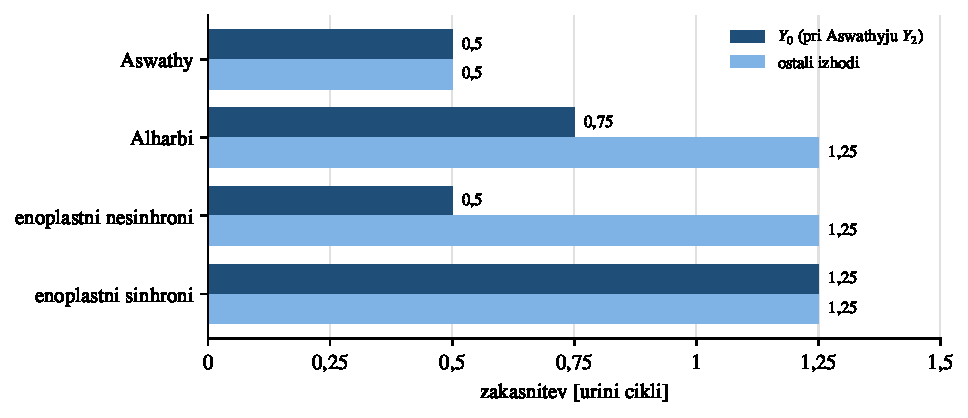
\includegraphics[width=\linewidth]{D4_zakasnitev}
\caption{Zakasnitev izhodov v urinih ciklih (enačba~\eqref{g21:eq:zakasnitev}). Pri Aswathyjevem vezju izhodu $Y_0$ ustreza izhod $Y_2$.}
\label{g21:fig:zakasnitev}
\end{figure}

Slika~\ref{g21:fig:valovne} prikazuje graf valovnih oblik sinhrone različice. Izhod $Y_0$ ima vrednost 1 le pri $S = \mathit{DATA} = 1$, $Y_1$ le pri $S = 0$ in $\mathit{DATA} = 1$, izhoda $\mathit{Scp}$ in $\mathit{DATAcp}$ pa sledita $\bar{S}$ oziroma $\mathit{DATA}$. Vezje torej za vse štiri kombinacije vhodov deluje pravilno. Impulzi vseh štirih izhodov so med seboj poravnani, kar potrjuje sinhronost.

\begin{figure}[htbp]
\centering
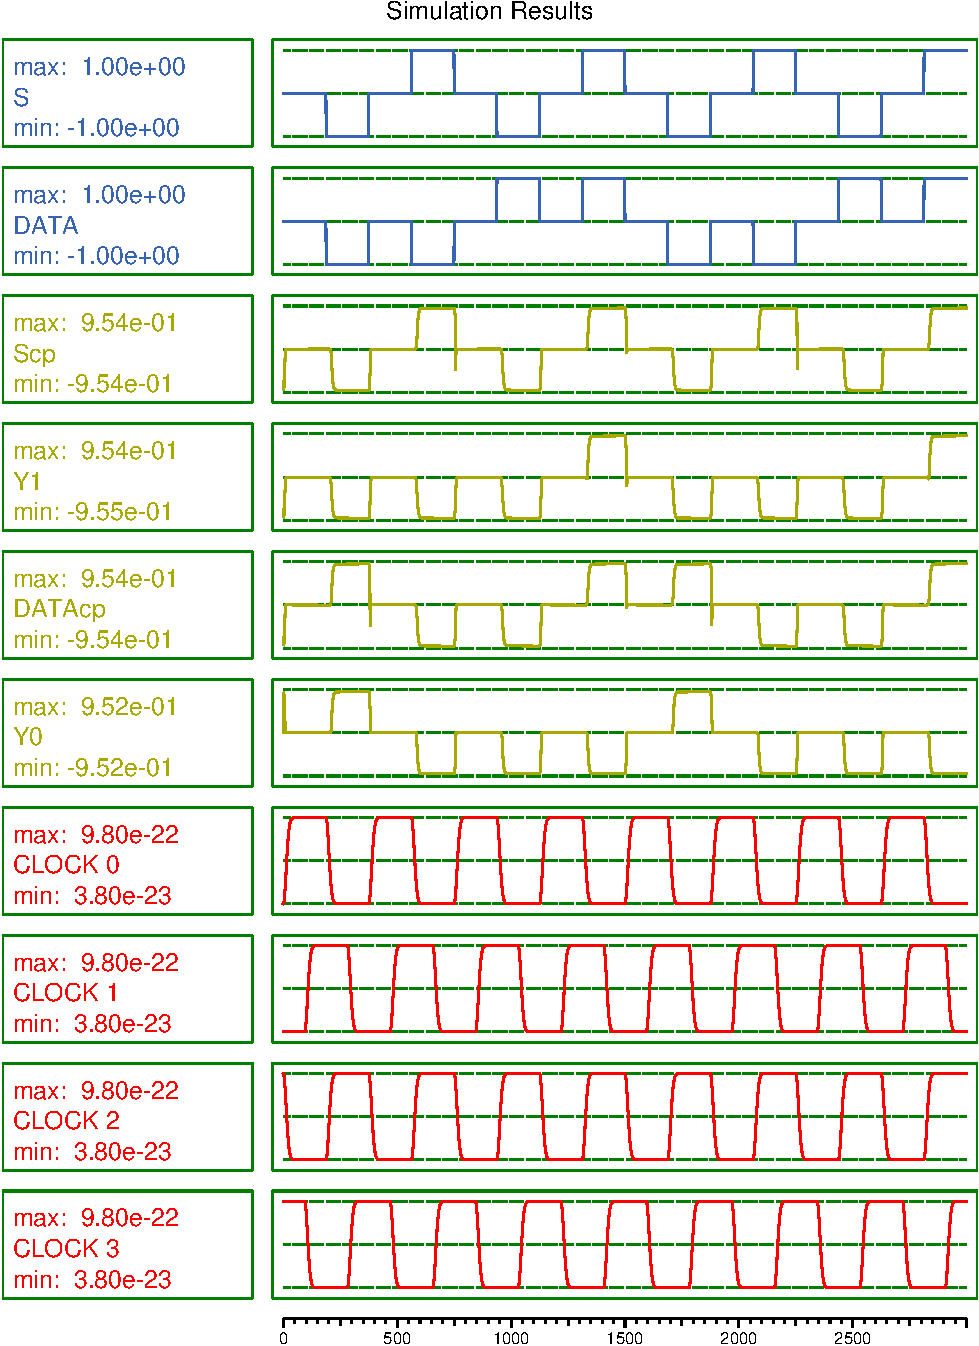
\includegraphics[width=\linewidth]{enoplastni_sinhroni_10ps}
\caption{Graf valovnih oblik sinhrone različice pri uri \SI{10}{\pico\second}. Vodoravna os prikazuje zaporedno številko vzorca, celoten graf pa obsega 8 urinih ciklov (\SI{800}{\pico\second}).}
\label{g21:fig:valovne}
\end{figure}

\subsection{Disipacija energije}
\label{g21:sec:poraba}

Slika~\ref{g21:fig:poraba} prikazuje disipacijo energije vseh vezij pri obeh hitrostih ure. Disipacija vseh treh reverzibilnih vezij je pri desetkrat počasnejši uri približno desetkrat manjša ($R$ med \num{9.3} in \num{9.7}), disipacija Aswathyjevega vezja pa ostane enaka ($R = \num{1.00}$). Rezultat je skladen s fizično reverzibilnostjo obeh lastnih različic. Ker smo disipacijo izmerili le pri dveh hitrostih ure, pa ne moremo potrditi, da se ob nadaljnjem upočasnjevanju ure približuje nič, kot bi pri fizično reverzibilnem vezju pričakovali. Pri \SI{100}{\pico\second} so vsa reverzibilna vezja pod Landauerjevo mejo, pri \SI{10}{\pico\second} pa le nesinhrona različica (\num{0.93}~$E_\mathrm{L}$). Aswathyjevo vezje je pri obeh hitrostih približno enajstkrat nad mejo.

\begin{figure}[htbp]
\centering
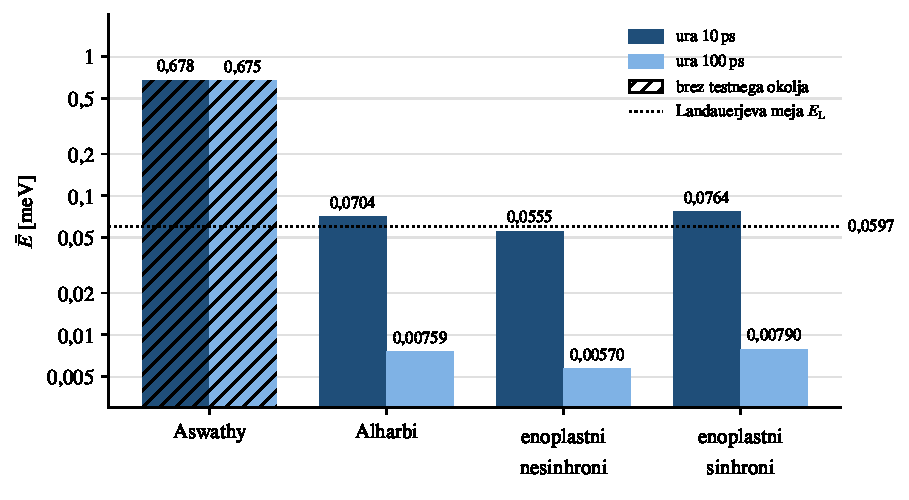
\includegraphics[width=\linewidth]{D1_poraba}
\caption{Povprečna disipacija na urin cikel $\bar{E}$ pri urah \SI{10}{\pico\second} in \SI{100}{\pico\second} (logaritemska os). Reverzibilna vezja so merjena s testnim okoljem, Aswathyjevo brez njega. Pikčasta črta označuje Landauerjevo mejo $E_\mathrm{L}$ (enačba~\eqref{g21:eq:landauer}).}
\label{g21:fig:poraba}
\end{figure}

Nesinhrona različica ima pri \SI{10}{\pico\second} za \SI{21}{\percent} manjšo disipacijo energije kot Alharbijevo vezje, pri \SI{100}{\pico\second} pa za \SI{25}{\percent} manjšo. Disipacija sinhrone različice je za \SI{9}{\percent} oziroma \SI{4}{\percent} večja kot pri Alharbijevem vezju in za približno \SI{38}{\percent} večja kot pri nesinhroni različici. Sinhronost izhodov ima torej opazno ceno v disipaciji energije.

Slika~\ref{g21:fig:testno} prikazuje vpliv testnega okolja. Brez njega je disipacija vseh treh reverzibilnih vezij okoli \SI{1.1}{\milli\electronvolt}, kar je več kot pri ireverzibilnem Aswathyjevem vezju (\SI{0.678}{\milli\electronvolt}). S počasnejšo uro se skoraj ne zmanjša ($R$ med \num{1.03} in \num{1.04}), zato se vezja brez testnega okolja obnašajo kot ireverzibilna. S testnim okoljem je disipacija 15- do 20-krat manjša. Skoraj vso disipacijo brez testnega okolja torej povzroči brisanje informacije na štirih izhodih, ki jih ne prevzame nobena celica.

\begin{figure}[htbp]
\centering
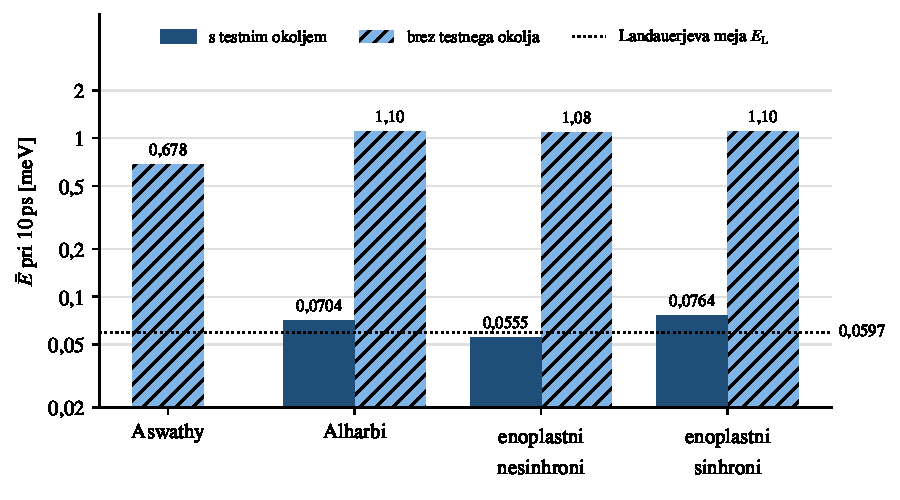
\includegraphics[width=\linewidth]{D2_testno_okolje}
\caption{Povprečna disipacija na urin cikel $\bar{E}$ pri uri \SI{10}{\pico\second} s testnim okoljem in brez njega (logaritemska os). Aswathyjevemu vezju testnega okolja ni mogoče dodati.}
\label{g21:fig:testno}
\end{figure}

Slika~\ref{g21:fig:celice} prikazuje, da disipacija reverzibilnih vezij približno sorazmerno narašča s številom računanih celic. Naklon premice skozi izhodišče, prilagojene po metodi najmanjših kvadratov, je približno \SI{1.27e-3}{\milli\electronvolt} na celico. Razlike v disipaciji med reverzibilnimi vezji torej izvirajo predvsem iz števila celic: nesinhrona različica jih ima najmanj, sinhrona pa največ zaradi podaljšane poti do $Y_0$. Ker simulator celice obravnava v naključnem vrstnem redu (\emph{Randomize Simulation Order}), ponovljena simulacija ne da povsem enakega rezultata. Ponovljena meritev Alharbijevega vezja pri \SI{10}{\pico\second} se od prve razlikuje za \SI{0.3}{\percent}, zato so razlike med vezji precej večje od razpršenosti meritev.

\begin{figure}[htbp]
\centering
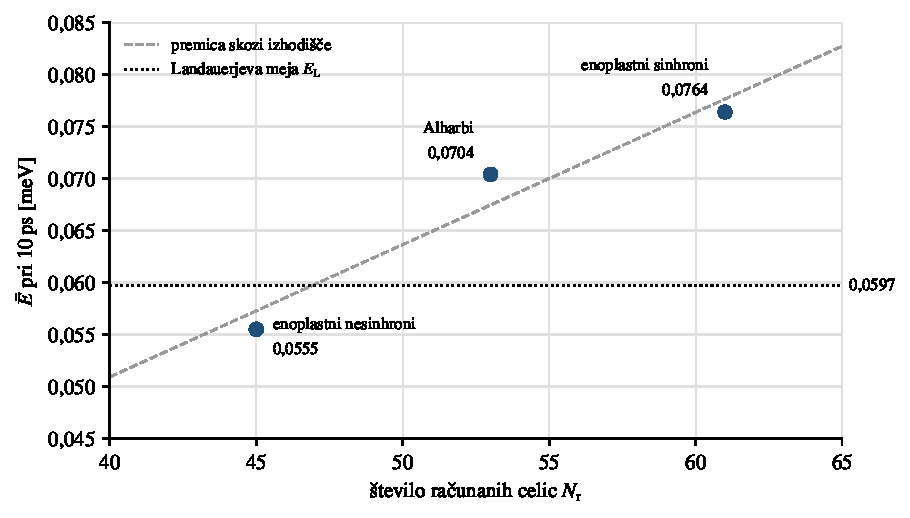
\includegraphics[width=\linewidth]{D3_celice}
\caption{Povprečna disipacija na urin cikel $\bar{E}$ pri uri \SI{10}{\pico\second} s testnim okoljem v odvisnosti od števila računanih celic $N_\mathrm{r}$. Črtkana črta je premica skozi izhodišče, prilagojena po metodi najmanjših kvadratov.}
\label{g21:fig:celice}
\end{figure}

\section{Razprava}
\label{g21:sec:razprava}

V okviru naloge smo implementirali štiri različice demultiplekserja 1:2: ireverzibilno vezje Aswathyja in sod. \cite{g21:aswathy2024}, fizično reverzibilno vezje Alharbija in sod. \cite{g21:alharbi2022} ter dve lastni enoplastni različici, nesinhrono in sinhrono.

Rezultati simulacij so pokazali, da je mogoče fizično reverzibilni demultiplekser realizirati v eni plasti, brez križanja vodil in s sinhronimi izhodi, pri čemer ohranja lastnosti fizične reverzibilnosti. Takšna zasnova poenostavi strukturo vezja in lahko izboljša stabilnost signalov, sinhronost izhodov pa omogoča njihovo sočasno uporabo v nadaljnjih vezjih. Pri tem je energijska disipacija sinhrone različice pri počasnejši uri le za približno 4\% večja od disipacije Alharbijevega vezja.

Vendar sinhrona različica ni v vseh pogledih boljša od nesinhrone. Med obravnavanimi reverzibilnimi vezji ima nesinhrona različica najmanjše število celic, najnižjo energijsko disipacijo in najnižjo ceno $C$, sinhrona pa pri vseh treh merilih dosega najvišje vrednosti. Izbira ustrezne različice je zato odvisna od zahtev in omejitev konkretne uporabe, saj nobena ni optimalna v vseh pogledih.

Ključna ugotovitev meritev je tudi, da se je pri vseh treh reverzibilnih vezjih energijska disipacija ob desetkrat počasnejši uri zmanjšala za približno desetkrat. Pri ireverzibilnem Aswathyjevem vezju \cite{g21:aswathy2024} je ostala skoraj nespremenjena. Takšno obnašanje dodatno podpira sklep o fizični reverzibilnosti Alharbijevega vezja \cite{g21:alharbi2022} in obeh lastnih različic.

Pri interpretaciji teh rezultatov je pomembno upoštevati tudi vpliv testnega okolja na energijsko disipacijo. Aswathyjevega vezja \cite{g21:aswathy2024} zaradi razporeditve celic okoli vhoda $S$ ni bilo mogoče dopolniti z medpomnilniškimi celicami, zato njegove energijske disipacije s testnim okoljem in brez njega nismo mogli primerjati. Pri preostalih treh vezjih pa smo lahko izvedli obe meritvi. Rezultati so pokazali, da je bila energijska disipacija brez testnega okolja bistveno večja in je ob upočasnitvi ure ostala skoraj nespremenjena. To nakazuje, da velik delež energijskih izgub izvira iz nepovratne izgube informacij na končnih izhodih. Pri realizaciji fizično reverzibilnih vezij moramo zato poskrbeti tudi za ohranjanje in ustrezen prenos izhodnih informacij v nadaljnje vezje.

\subsection{Kaj ni delovalo}
\label{g21:sec:neuspehi}

Med izvajanjem seminarske naloge smo naleteli tudi na nekatere omejitve. Zaradi že omenjenih težav pri dodajanju testnega okolja Aswathyjevemu vezju \cite{g21:aswathy2024} njegove energijske disipacije ni bilo mogoče neposredno primerjati z energijsko disipacijo ostalih vezij pod enakimi pogoji. 

Prav tako se je pri rekonstrukciji Alharbijevega vezja \cite{g21:alharbi2022} izmerjena energijska disipacija razlikovala od vrednosti, navedene v izvornem članku, za približno 26\%. Natančnega vzroka za odstopanje nismo ugotovili, vendar so se drugi preverjeni parametri vezja, vključno z zakasnitvami izhodov in številom ploščic, ujemali z objavljenimi rezultati.

\section{Zaključek}
\label{g21:sec:zakljucek}

V seminarski nalogi smo predstavili in primerjali štiri različice demultiplekserja 1:2 v QCA. Cilj naloge je bil poenostaviti in izboljšati vezje Alharbija in sod.~\cite{g21:alharbi2022} ter pri tem ohranjati fizično reverzibilnost. 

S prvo lastno različico smo odpravili večplastno križanje vodil, vendar so izhodi ostali nesinhroni. V drugi različici smo dosegli sinhronost vseh izhodov ob ohranitvi enoplastne izvedbe in lastnosti fizične reverzibilnosti. Sinhronizacija izhodov je zahtevala več celic, kar je povečalo površino vezja in energijsko disipacijo. Kljub tem kompromisom rezultati simulacij kažejo, da je mogoče zasnovati enoplastni fizično reverzibilni demultiplekser s sinhronimi izhodi. 

V nadaljnjem delu bi bilo smiselno vezja simulirati pri več različnih hitrostih ure, s čimer bi lahko dodatno preverili njihovo fizično reverzibilnost. Možna izboljšava je tudi optimizacija sinhrone različice z drugačno razporeditvijo celic in urinih con, da bi zmanjšali njeno površino in energijsko disipacijo ter pri tem ohranili sinhronost izhodov in skladnost s ploščicami $5\times5$.

\section*{Doprinosi avtorjev}

Jaka Pelko je pregledal obstoječe izvedbe demultiplekserjev v QCA. V QCADesigner-E je implementiral referenčni in lastni vezji ter izvedel simulacije.

Miha Vintar je sodeloval pri pisanju poročila. Napisal je skripto za izris grafov in pripravil slike~\ref{g21:fig:zakasnitev} in~\ref{g21:fig:poraba} do \ref{g21:fig:celice}.

Tara Majkič je sodelovala pri pisanju poročila. Pripravila je prosojnice, v katerih je povzela potek dela in rezultate.

\section*{Izjava o uporabi generativne umetne inteligence}

Uporabili smo orodji ChatGPT in Claude. Z njimi smo si pomagali pri pregledu področja, pri lektoriranju poročila ter pri odpravljanju težav s programom QCADesigner-E.
